\documentclass[10pt]{article}
\usepackage{amsmath, amssymb, amsthm, tikz}
\usepackage[top=2cm, left = 2cm, right = 2cm, bottom = 3cm]{geometry}
%\usepackage[pdftex]{graphicx}
\usepackage{fancyhdr}
\newcommand{\proposed}[1]
{
\vspace{5pt}
\noindent\textit{Proposed by #1}
}
\newcommand{\solution}
{
\vspace{5pt}
\noindent\textit{Solution.}\qquad
}
\providecommand{\abs}[1]{\left\vert#1\right\vert}

\pagestyle{fancy}
\rhead{}
\chead{\includegraphics[scale=0.12]{CMIMC-header.png}}
\lhead{}
\setlength{\headheight}{43pt}
\rfoot{}
\cfoot{}
\lfoot{}
\begin{document}

\begin{center}
\huge\textbf{Computer Science Solutions Packet}\normalsize

\vspace{3pt}
\end{center}

\begin{enumerate}
\setlength{\itemsep}{3pt}

\item For how many distinct ordered triples $(a,b,c)$ of boolean variables does the expression $a \lor (b \land c)$ evaluate to true?

\proposed{Cody Johnson}

\solution If $a$ is true, then we can have four assignments of $(b \land c)$, since $(b \land c)$ can be anything. If $a$ is false, then we can have one assignment of $(b \land c)$, since $(b \land c)$ must be true. Thus, the total number of distinct ordered triples of boolean variables that make the expression evaluate to true is $\boxed{5}$. 

\item In concurrent computing, two processes may have their steps interwoven in an unknown order, as long as the steps of each process occur in order. Consider the following two processes:

\begin{center}
\begin{tabular}{c|cc}
Process & $A$ & $B$\\
\hline
Step 1 & $x\leftarrow x-4$ & $x\leftarrow x-5$\\
Step 2 & $x\leftarrow x\cdot3$ & $x\leftarrow x\cdot4$\\
Step 3 & $x\leftarrow x-4$ & $x\leftarrow x-5$\\
Step 4 & $x\leftarrow x\cdot3$ & $x\leftarrow x\cdot4$
\end{tabular}
\end{center}

One such interweaving is $A1$, $B1$, $A2$, $B2$, $A3$, $B3$, $B4$, $A4$, but $A1$, $A3$, $A2$, $A4$, $B1$, $B2$, $B3$, $B4$ is not since the steps of $A$ do not occur in order. We run $A$ and $B$ concurrently with $x$ initially valued at $6$. Find the minimal possible value of $x$ among all interweavings.

\proposed{Joshua Siktar}

\solution Consider the first two steps of $A$ and $B$. Be it $A$ or $B$, we must execute some step 2 within the first three steps of the concurrent process. Since we multiply $x$ by a positive number in either step 2, we would like to minimize $x$ before it is multiplied. Thus, we execute step 1 of both $A$ and $B$ first, which gives us $x = (6-4)-5 = -3$ in the first two steps of the concurrent process. 

\par Now, we must multiply $x$ by 3 or 4, which makes the absolute value of $x$ at least 9. Thus, multiplying later will beat the $x$ that we multiply early. So, we know that steps 4 of $A$ and $B$ will come last. 

\par We just need to figure out how to execute steps 2 and 3. If we execute steps 2 of $A$ and $B$ first, we get $(-3\cdot 3\cdot 4) - 4 - 5 = -45$. If we execute step 2 of $A$ first, we get $(-3\cdot 3 - 4)\cdot 4 - 5 = -57$. If we execute step 2 of $B$ first, we get $(-3\cdot 4 - 5)\cdot 3 - 4 = -55$. 

\par Thus, we choose to execute step 2 of $A$ first and achieve a minimum value of $x$ of $-57\cdot 3\cdot 4 = \boxed{-684}$. 

\item Sophia writes an algorithm to solve the graph isomorphism problem. Given a graph $G=(V,E)$, her algorithm iterates through all permutations of the set $\{v_1, \dots, v_{|V|}\}$, each time examining all ordered pairs $(v_i,v_j)\in V\times V$ to see if an edge exists. When $|V|=8$, her algorithm makes $N$ such examinations. What is the largest power of two that divides $N$?

\proposed{Cody Johnson}

\solution If $n := |V_1|$, then the number of pairs of vertices $(u,v)$ is
$n^2$. The number of bijections $\phi: V_1 \to V_2$ is $n!$ when $|V_1| =
|V_2|$, so we have must test for $n^2\cdot n!$ pairs of vertices. Let
$v_{2}(m)$ be the highest power of $2$ dividing $m$. Then, when $n = 8$, then $N = 8^2\cdot 8!$ and the largest integer $k$ such that $N/2^k$ is an integer is \begin{align*}k &= v_2(8^2) + v_2(8!) \\&= 6 + \left\lfloor \frac82 \right\rfloor + \left\lfloor \frac84 \right\rfloor + \left\lfloor \frac88 \right\rfloor \\&= 6 + 4 + 2 + 1 = \boxed{13}.\end{align*}  (We will also accept $2^{13} = 8192$.)

\item Given a list $A$, let $f(A) = [A[0] + A[1], A[0] - A[1]]$. Alef makes two programs to compute $f(f(...(f(A))))$, where the function is composed $n$ times:

\begin{center}
\begin{tabular}{l|l}
1: \textbf{FUNCTION} $T_1(A, n)$ & 1: \textbf{FUNCTION} $T_2(A, n)$ \\
2: $\quad$ \textbf{IF} $n = 0$ & 2: $\quad$ \textbf{IF} $n = 0$ \\
3: $\quad$ $\quad$  \textbf{RETURN} $A$ & 3: $\quad$ $\quad$ \textbf{RETURN} $A$ \\
4: $\quad$ \textbf{ELSE} & 4: $\quad$ \textbf{ELSE} \\
5: $\quad$ $\quad$  \textbf{RETURN} $[T_1(A, n - 1)[0] + T_1(A, n - 1)[1],$ & 5: $\quad$ $\quad$ $B \leftarrow T_2(A, n - 1)$ \\
$\quad$ $\quad$ $\quad$ $T_1(A, n - 1)[0] - T_1(A, n - 1)[1]]$ & 6: $\quad$ $\quad$ \textbf{RETURN} $[B[0] + B[1], B[0] - B[1]]$ \\

\end{tabular}
\end{center}

Each time $T_1$ or $T_2$ is called, Alef has to pay one dollar. How much money does he save by calling $T_2([13, 37], 4)$ instead of $T_1([13, 37], 4)$?

\proposed{Cody Johnson}

\solution If Alef uses $T_1$, then \[T_1(A,n) = 4(T_1(B,n-1)+1) = 4(4(T_1(C,n-2)+1)+1) = \cdots = \sum_{i=0}^n 4^i.\] Thus, \[T_1([13,37],4) =  1+4 + 4^2 + 4^3 + 4^4 = 341.\] In a similar fashion, we can write \[T_2(A,n) = T_2(B,n-1)+1 = (T_2(C,n-2)+1)+1 = \cdots = n + 1.\] Thus, the difference is $341 - 5 = \boxed{336}$. 

\item We define the \emph{weight} of a path to be the sum of the numbers written on each edge of the path. Find the minimum weight among all paths in the graph below that visit each vertex precisely once:

\begin{center}
\begin{tikzpicture}
\draw (-1,-3)--(1,-1)--(2,-2)--(0,-4)--(-2,-2)--(0,0)--(1,-1);
\draw (-1,-1)--(-1,-3)--(1,-3)--(1,-1)--(-1,-1)--(1,-3);

\node [circle,fill=black] at (0,0) {};
\node [circle,fill=black] at (-1,-1) {};
\node [circle,fill=black] at (1,-1) {};
\node [circle,fill=black] at (-2,-2) {};
\node [circle,fill=black] at (0,-2) {};
\node [circle,fill=black] at (2,-2) {};
\node [circle,fill=black] at (-1,-3) {};
\node [circle,fill=black] at (1,-3) {};
\node [circle,fill=black] at (0,-4) {};

\node [above left] at (-0.5,-0.5) {$9$};
\node [above left] at (-1.5,-1.5) {$3$};
\node [above right] at (0.5,-0.5) {$16$};
\node [above right] at (1.5,-1.5) {$11$};
\node [below left] at (-1.5,-2.5) {$19$};
\node [below left] at (-0.5,-3.5) {$3$};
\node [below right] at (1.5,-2.5) {$17$};
\node [below right] at (0.5,-3.5) {$14$};
\node [above] at (0,-1) {$11$};
\node [left] at (-1,-2) {$20$};
\node [right] at (1,-2) {$18$};
\node [below] at (0,-3) {$6$};
\node at (-0.45,-1.3) {$4$};
\node at (0.45,-1.3) {$4$};
\node at (-0.45,-2.65) {$8$};
\node at (0.45,-2.65) {$2$};
\end{tikzpicture}
\end{center}

\proposed{Cody Johnson}

\solution
Very easy casework shows that up to rotation and reflection, there are three types of paths in total, of the following forms:

\begin{center}
\begin{tikzpicture}[scale=0.25]
\draw (0,0)--(-2,-2)--(0,-4)--(2,-2)--(1,-1)--(0,-2);
\draw (6,0)--(4,-2)--(6,-4)--(7,-3)--(6,-2)--(7,-1)--(8,-2);
\draw (12,0)--(10,-2)--(11,-3)--(13,-1)--(14,-2)--(12,-4);
\end{tikzpicture}
\end{center}

Among all paths of the first kind, the one with the minimal weight has weight

$$16+11+17+14+3+19+3+9+\min\{4-\max\{16,11\},2-\max\{17,14\},\dots\}$$

which is $77$ by inspection. Among all paths of the second kind, the one with the minimal weight has weight

$$\min\{9+3+19+3+4+2+\min\{16+17,11+14\},3+9+16+11+8+2+\min\{19+14,3+17\},\dots\}$$

which is $65$ by inspection. Among all paths of the third kind, the one with the minimal weight has weight

$$\min\{3+9+8+4+14+17+\min\{3+16,19+11\},16+11+4+2+3+19+\min\{9+14,3+17\}\}$$

which is $74$ by inspection. Thus, the minimum weight spanning path has weight $\boxed{65}$. 

\item Aaron is trying to write a program to compute the terms of the sequence defined recursively by $a_0=0$, $a_1=1$, and \[a_n=\begin{cases}a_{n-1}-a_{n-2}&n\equiv0\pmod2\\2a_{n-1}-a_{n-2}&\text{else}\end{cases}\] However, Aaron makes a typo, accidentally computing the recurrence by \[a_n=\begin{cases}a_{n-1}-a_{n-2}&n\equiv0\pmod3\\2a_{n-1}-a_{n-2}&\text{else}\end{cases}\] For how many $0\le k\le2016$ did Aaron coincidentally compute the correct value of $a_k$?

\proposed{Cody Johnson}

\solution Note that the values of $a_k$, the values computed by the original program, and the values of $a'_k$, the values computed by the program with the typo, are periodic: the original program repeats the sequence $0,1,1,1,1,0,-1,-1,-1$ and the program with the typo repeats the sequence $0,1,2,1,0,-1,-1,-1,-1$. Since the elements of $a_k$ have a period of length 8 and the elements of $a'_k$ has a period of length 9, we just need to count the number of coincidences in the first $8\cdot 9 = 72$ terms of $a_k$ and $a'_k$, since 8 and 9 are coprime. When the beginnings of the periodic segments of $a_k$ and $a'_k$ are 0 off, there are $7$ coincidences. When they are 1 off, there are $3$ coincidences. When they are 2 off, there are $2$. When they are 3 off, there are $0$. When they are 4 off, there are $2$. When they are $5$ off, there are $1$. When they are $6$ off, there are $3$. When they are $7$ off, there are $4$. Thus, in the first 72 terms, Aaron accidnetally computes the correct values of $a_k$ for $7+3+2+0+2+1+3+4 = 22$ values. Thus, for $0 \leq k \leq 2016$, he correctly computes $2016 / 72 \cdot 22 = 28 \cdot 22 = \boxed{616}$ values. 

\item Given the list \[A=[9,12,1,20,17,4,10,7,15,8,13,14],\] we would like to sort it in increasing order.  To accomplish this, we will perform the following operation repeatedly: remove an element, then insert it at any position in the list, shifting elements if necessary.  What is the minimum number of applications of this operation necessary to sort $A$?

\proposed{Cody Johnson}

\solution Observation: for each pair that is out of order (like $(12,1)$), at least one of the elements must be swapped using the algorithm. From this observation, we draw a graph $G$ with vertices representing the elements of $A$, and an edge between each pair of vertices that is initially out of order (so the vertex for $12$ is connected to the vertex for $1$). Due to the observation, the minimum is at least the size of the minimal vertex cover of $G$.

\begin{center}
\begin{tikzpicture}[scale=1/2.5]
\node (G) at (10,0) {};
\node (F) at (8.66025403784,5) {};
\node (E) at (5,8.66025403784) {};
\node (D) at (0,10) {};
\node (C) at (-5,8.66025403784) {};
\node (B) at (-8.66025403784,5) {};
\node (A) at (-10,0) {};
\node (L) at (-8.66025403784,-5) {};
\node (K) at (-5,-8.66025403784) {};
\node (J) at (0,-10) {};
\node (I) at (5,-8.66025403784) {};
\node (H) at (8.66025403784,-5) {};

\draw (A)--(C);
\draw (A)--(F);
\draw (A)--(H);
\draw (A)--(J);
\draw (B)--(C);
\draw (B)--(F);
\draw (B)--(G);
\draw (B)--(H);
\draw (B)--(J);
\draw (D)--(E);
\draw (D)--(F);
\draw (D)--(G);
\draw (D)--(H);
\draw (D)--(I);
\draw (D)--(J);
\draw (D)--(K);
\draw (D)--(L);
\draw (E)--(F);
\draw (E)--(G);
\draw (E)--(H);
\draw (E)--(I);
\draw (E)--(J);
\draw (E)--(K);
\draw (E)--(L);
\draw (G)--(H);
\draw (G)--(J);
\draw (I)--(J);
\draw (I)--(K);
\draw (I)--(L);

\node [circle,fill=white,draw] at (A) {$9$};
\node [circle,fill=white,draw] at (B) {$12$};
\node [circle,fill=white,draw] at (C) {$1$};
\node [circle,fill=white,draw] at (D) {$20$};
\node [circle,fill=white,draw] at (E) {$17$};
\node [circle,fill=white,draw] at (F) {$4$};
\node [circle,fill=white,draw] at (G) {$10$};
\node [circle,fill=white,draw] at (H) {$7$};
\node [circle,fill=white,draw] at (I) {$15$};
\node [circle,fill=white,draw] at (J) {$8$};
\node [circle,fill=white,draw] at (K) {$13$};
\node [circle,fill=white,draw] at (L) {$14$};
\end{tikzpicture}
\end{center}

Let $n$ be the size of a minimal vertex cover of $G$. We claim $n=6$. One such cover is the set $\{20,17,12,9,15,10\}$. Let $S$ be a minimal vertex cover of $G$. Note that $\deg\{20\}=8>6$, so $20\in S$. Also, after deleting $20$, $\deg\{17\}=7>5$, so $17\in S$. After deleting $17$, $\deg\{12\}=5>4$, so $12\in S$. Then $\deg\{9\}=4>3$, so $9\in S$. Then $\deg\{15\}=3>2$, so $15\in S$. Finally, $\deg\{10\}=2>1$, so $10\in S$. This is already a vertex cover. (This deletion process is described in the diagram below)

\begin{center}
\begin{tikzpicture}[scale=1/7.5]
\node (G) at (10,0) {};
\node (F) at (8.66025403784,5) {};
\node (E) at (5,8.66025403784) {};
\node (D) at (0,10) {};
\node (C) at (-5,8.66025403784) {};
\node (B) at (-8.66025403784,5) {};
\node (A) at (-10,0) {};
\node (L) at (-8.66025403784,-5) {};
\node (K) at (-5,-8.66025403784) {};
\node (J) at (0,-10) {};
\node (I) at (5,-8.66025403784) {};
\node (H) at (8.66025403784,-5) {};

\draw (A)--(C);
\draw (A)--(F);
\draw (A)--(H);
\draw (A)--(J);
\draw (B)--(C);
\draw (B)--(F);
\draw (B)--(G);
\draw (B)--(H);
\draw (B)--(J);
\draw (D)--(E);
\draw (D)--(F);
\draw (D)--(G);
\draw (D)--(H);
\draw (D)--(I);
\draw (D)--(J);
\draw (D)--(K);
\draw (D)--(L);
\draw (E)--(F);
\draw (E)--(G);
\draw (E)--(H);
\draw (E)--(I);
\draw (E)--(J);
\draw (E)--(K);
\draw (E)--(L);
\draw (G)--(H);
\draw (G)--(J);
\draw (I)--(J);
\draw (I)--(K);
\draw (I)--(L);

\draw [fill=black] (A) circle (0.5cm);
\draw [fill=black] (B) circle (0.5cm);
\draw [fill=black] (C) circle (0.5cm);
\draw [fill=black] (D) circle (0.5cm);
\draw [fill=black] (E) circle (0.5cm);
\draw [fill=black] (F) circle (0.5cm);
\draw [fill=black] (G) circle (0.5cm);
\draw [fill=black] (H) circle (0.5cm);
\draw [fill=black] (I) circle (0.5cm);
\draw [fill=black] (J) circle (0.5cm);
\draw [fill=black] (K) circle (0.5cm);
\draw [fill=black] (L) circle (0.5cm);
\end{tikzpicture}
\hspace{1cm}
\begin{tikzpicture}[scale=1/7.5]
\node (G) at (10,0) {};
\node (F) at (8.66025403784,5) {};
\node (E) at (5,8.66025403784) {};
\node (D) at (0,10) {};
\node (C) at (-5,8.66025403784) {};
\node (B) at (-8.66025403784,5) {};
\node (A) at (-10,0) {};
\node (L) at (-8.66025403784,-5) {};
\node (K) at (-5,-8.66025403784) {};
\node (J) at (0,-10) {};
\node (I) at (5,-8.66025403784) {};
\node (H) at (8.66025403784,-5) {};

\draw (A)--(C);
\draw (A)--(F);
\draw (A)--(H);
\draw (A)--(J);
\draw (B)--(C);
\draw (B)--(F);
\draw (B)--(G);
\draw (B)--(H);
\draw (B)--(J);
\draw (E)--(F);
\draw (E)--(G);
\draw (E)--(H);
\draw (E)--(I);
\draw (E)--(J);
\draw (E)--(K);
\draw (E)--(L);
\draw (G)--(H);
\draw (G)--(J);
\draw (I)--(J);
\draw (I)--(K);
\draw (I)--(L);

\draw [fill=black] (A) circle (0.5cm);
\draw [fill=black] (B) circle (0.5cm);
\draw [fill=black] (C) circle (0.5cm);
\draw [fill=black] (E) circle (0.5cm);
\draw [fill=black] (F) circle (0.5cm);
\draw [fill=black] (G) circle (0.5cm);
\draw [fill=black] (H) circle (0.5cm);
\draw [fill=black] (I) circle (0.5cm);
\draw [fill=black] (J) circle (0.5cm);
\draw [fill=black] (K) circle (0.5cm);
\draw [fill=black] (L) circle (0.5cm);
\end{tikzpicture}
\hspace{1cm}
\begin{tikzpicture}[scale=1/7.5]
\node (G) at (10,0) {};
\node (F) at (8.66025403784,5) {};
\node (E) at (5,8.66025403784) {};
\node (D) at (0,10) {};
\node (C) at (-5,8.66025403784) {};
\node (B) at (-8.66025403784,5) {};
\node (A) at (-10,0) {};
\node (L) at (-8.66025403784,-5) {};
\node (K) at (-5,-8.66025403784) {};
\node (J) at (0,-10) {};
\node (I) at (5,-8.66025403784) {};
\node (H) at (8.66025403784,-5) {};

\draw (A)--(C);
\draw (A)--(F);
\draw (A)--(H);
\draw (A)--(J);
\draw (B)--(C);
\draw (B)--(F);
\draw (B)--(G);
\draw (B)--(H);
\draw (B)--(J);
\draw (G)--(H);
\draw (G)--(J);
\draw (I)--(J);
\draw (I)--(K);
\draw (I)--(L);

\draw [fill=black] (A) circle (0.5cm);
\draw [fill=black] (B) circle (0.5cm);
\draw [fill=black] (C) circle (0.5cm);
\draw [fill=black] (F) circle (0.5cm);
\draw [fill=black] (G) circle (0.5cm);
\draw [fill=black] (H) circle (0.5cm);
\draw [fill=black] (I) circle (0.5cm);
\draw [fill=black] (J) circle (0.5cm);
\draw [fill=black] (K) circle (0.5cm);
\draw [fill=black] (L) circle (0.5cm);
\end{tikzpicture}
\end{center}

\begin{center}
\begin{tikzpicture}[scale=1/7.5]
\node (G) at (10,0) {};
\node (F) at (8.66025403784,5) {};
\node (E) at (5,8.66025403784) {};
\node (D) at (0,10) {};
\node (C) at (-5,8.66025403784) {};
\node (B) at (-8.66025403784,5) {};
\node (A) at (-10,0) {};
\node (L) at (-8.66025403784,-5) {};
\node (K) at (-5,-8.66025403784) {};
\node (J) at (0,-10) {};
\node (I) at (5,-8.66025403784) {};
\node (H) at (8.66025403784,-5) {};

\draw (A)--(C);
\draw (A)--(F);
\draw (A)--(H);
\draw (A)--(J);
\draw (G)--(H);
\draw (G)--(J);
\draw (I)--(J);
\draw (I)--(K);
\draw (I)--(L);

\draw [fill=black] (A) circle (0.5cm);
\draw [fill=black] (C) circle (0.5cm);
\draw [fill=black] (F) circle (0.5cm);
\draw [fill=black] (G) circle (0.5cm);
\draw [fill=black] (H) circle (0.5cm);
\draw [fill=black] (I) circle (0.5cm);
\draw [fill=black] (J) circle (0.5cm);
\draw [fill=black] (K) circle (0.5cm);
\draw [fill=black] (L) circle (0.5cm);
\end{tikzpicture}
\hspace{1cm}
\begin{tikzpicture}[scale=1/7.5]
\node (G) at (10,0) {};
\node (F) at (8.66025403784,5) {};
\node (E) at (5,8.66025403784) {};
\node (D) at (0,10) {};
\node (C) at (-5,8.66025403784) {};
\node (B) at (-8.66025403784,5) {};
\node (A) at (-10,0) {};
\node (L) at (-8.66025403784,-5) {};
\node (K) at (-5,-8.66025403784) {};
\node (J) at (0,-10) {};
\node (I) at (5,-8.66025403784) {};
\node (H) at (8.66025403784,-5) {};


\draw (G)--(H);
\draw (G)--(J);
\draw (I)--(J);
\draw (I)--(K);
\draw (I)--(L);

\draw [fill=black] (C) circle (0.5cm);
\draw [fill=black] (F) circle (0.5cm);
\draw [fill=black] (G) circle (0.5cm);
\draw [fill=black] (H) circle (0.5cm);
\draw [fill=black] (I) circle (0.5cm);
\draw [fill=black] (J) circle (0.5cm);
\draw [fill=black] (K) circle (0.5cm);
\draw [fill=black] (L) circle (0.5cm);
\end{tikzpicture}
\hspace{1cm}\begin{tikzpicture}[scale=1/7.5]
\node (G) at (10,0) {};
\node (F) at (8.66025403784,5) {};
\node (E) at (5,8.66025403784) {};
\node (D) at (0,10) {};
\node (C) at (-5,8.66025403784) {};
\node (B) at (-8.66025403784,5) {};
\node (A) at (-10,0) {};
\node (L) at (-8.66025403784,-5) {};
\node (K) at (-5,-8.66025403784) {};
\node (J) at (0,-10) {};
\node (I) at (5,-8.66025403784) {};
\node (H) at (8.66025403784,-5) {};


\draw (G)--(H);
\draw (G)--(J);

\draw [fill=black] (C) circle (0.5cm);
\draw [fill=black] (F) circle (0.5cm);
\draw [fill=black] (G) circle (0.5cm);
\draw [fill=black] (H) circle (0.5cm);
\draw [fill=black] (J) circle (0.5cm);
\draw [fill=black] (K) circle (0.5cm);
\draw [fill=black] (L) circle (0.5cm);
\end{tikzpicture}
\end{center}

Now we show that $6$ is obtained as the solution to the original problem. Consider the following sequence of operations:

\[A=[9, 12, 1, 20, 17, 4, 10, 7, 15, 8, 13, 14]\]
\[A=[12, 1, 20, 17, 4, 10, 7, 15, 8, 9, 13, 14]\]
\[A=[1, 20, 17, 4, 10, 7, 15, 8, 9, 12, 13, 14]\]
\[A=[1, 17, 4, 10, 7, 15, 8, 9, 12, 13, 14, 20]\]
\[A=[1, 4, 10, 7, 15, 8, 9, 12, 13, 14, 17, 20]\]
\[A=[1, 4, 7, 15, 8, 9, 10, 12, 13, 14, 17, 20]\]
\[A=[1, 4, 7, 8, 9, 10, 12, 13, 14, 15, 17, 20]\]

Thus, the correct answer is $\boxed{6}$. 

\item Consider the sequence of sets defined by $S_0=\{0,1\},S_1=\{0,1,2\}$, and for $n\ge2$, \[S_n=S_{n-1}\cup\{2^n+x\mid x\in S_{n-2}\}.\] For example, $S_2=\{0,1,2\}\cup\{2^2+0,2^2+1\}=\{0,1,2,4,5\}$. Find the $200$th smallest element of $S_{2016}$.

\proposed{Cody Johnson}

\solution Note that for any $n$, the elements of $S_{n-1}$ will all be less than
the elements of $\{2^n + x \mid S_{n-2}\}$. Thus, the 200th smallest element of
$S_{2016}$ will also be the 200th smallest element of any $S_i$ such that the
cardinality of $S_i$ is at least 200. Let $\abs{\cdot}$ denote the cardinality
of a set. Then, also note that the sequence of $\abs{S_i}$ is the Fibonacci
sequence starting from 2, since $S_{n-1}$ and $\{2^n + x \mid S_{n-2}\}$ are
disjoint for all $n$. Thus, we look for the 200th smallest element in the $S_k$
such that $k$ is the smallest number such that the $k$th Fibonacci number is
larger than 200. We see that $k = 10$, which corresponds to the Fibonacci number
233, satisfies this. Then, the 200th smallest element of $S_{10}$ will be
$2^{10} + x$, where $x$ is the $200-144=56$th smallest element in $S_8$. The
56th smallest element in $S_8$ is just $2^8 + 0$, since $\abs{S_7} = 55$. Thus,
the 200th smallest number element in $S_{2016}$ is $2^{10} + 2^6 = 1024 + 256 =
\boxed{1280}$. 

\item Ryan has three distinct eggs, one of which is made of rubber and thus
	cannot break; unfortunately, he doesn't know which egg is the rubber
	one. Further, in some 100-story building there exists a floor such that
	all normal eggs dropped from below that floor will not break, while
	those dropped from at or above that floor will break and cannot be
	dropped again. What is the minimum number of times Ryan must drop an egg to determine the floor satisfying this property?

\proposed{Cody Johnson}

\solution Here is a strategy to obtain $\boxed{24}$: drop one egg, until it breaks, from floors $12$, $12+12$, $12+12+11$, $12+12+11+11$, $\dots$, $12+12+\dots+8+8$. If it never breaks, then the egg was fake and thus it reduces to the $100$-floor, two-egg problem. If it breaks on some floor, then drop both eggs on each floor from the bottom up until an egg breaks. It’s easy to calculate that this strategy will use either $23$ or $24$ drops in all of the cases.

Now, given any optimal strategy, we can modify it into another optimal strategy so that the strategy consists of iteratively dropping only one egg. Therefore, it suffices to find an increasing sequence of floors $1\le a_1<a_2<\dots<a_{n-1}<100\le a_n$ that is optimal.

If the egg never breaks then we have made $n$ drops, so we will finish in $n+14$ drops. If an egg drops on floor $a_k$, then we will necessarily need $2(a_k - 1 - a_{k-1})$ more drops. Thus, we want to minimize \[\max\{n+14,1+2(a_1-1),2+2(a_2-a_1-1),\dots,n+2(a_n-a_{n-1}-1)\}.\] By the averaging principle, we have \[\max\{1+2(a_1-1),2+2(a_2-a_1-1),\dots,n+2(a_n-a_{n-1}-1)\}\ge\frac{n(n+1)/2+2(a_n-n)}n\ge\frac{n(n+1)/2+2(100-n)}n.\] When $n\le9$, this is $\ge24$. When $n\ge11$, $n+14>24$. Therefore, $n=10$, which already means the maximum is at least $24$.

\item Given $x_0\in\mathbb R$, $f,g:\mathbb R\to\mathbb R$, we define the \emph{non-redundant binary tree} $T(x_0,f,g)$ in the following way:

\begin{enumerate}
\item The tree $T$ initially consists of just $x_0$ at height $0$.

\item Let $v_0,\dots,v_k$ be the vertices at height $h$. Then the vertices of height $h+1$ are added to $T$ by: for $i=0,1,\dots,k$, $f(v_i)$ is added as a child of $v_i$ if $f(v_i)\not\in T$, and $g(v_i)$ is added as a child of $v_i$ if $g(v_i)\not\in T$.
\end{enumerate}

For example, if $f(x)=x+1$ and $g(x)=x-1$, then the first three layers of $T(0,f,g)$ look like:

\begin{center}
\begin{tikzpicture}
\draw [->] (-0.1,-0.2)--(-0.4,-0.8);
\draw [->] (0.1,-0.2)--(0.4,-0.8);
\draw [->] (-0.6,-1.2)--(-0.9,-1.8);
\draw [->] (0.6,-1.2)--(0.9,-1.8);

\node at (0,0) {$0$};
\node at (-.5,-1) {$1$};
\node at (.5,-1) {$-1$};
\node at (-1,-2) {$2$};
\node at (1,-2) {$-2$};
\end{tikzpicture}
\end{center}

If $f(x)=1024x-2047\lfloor x/2\rfloor$ and $g(x)=2x-3\lfloor x/2\rfloor+2\lfloor x/4\rfloor$, then how many vertices are in $T(2016,f,g)$?

\proposed{Cody Johnson}

\solution First we change $f,g$ to binary string operations. For the first one, note that $f(x)=2^{10}(x-\lfloor x/2\rfloor)+\lfloor x/2\rfloor$, which, for strings of length $\le11$, transforms the string of digits $d_{10}\dots d_1d_0\to d_0d_{10}\dots d_1$, preserving that the length is $\le11$. For the second one, note that $f(x)=x+(x-2\lfloor x/2\rfloor)-(\lfloor x/2\rfloor-2\lfloor x/4\rfloor)$. If $x$ is an integer $\equiv0,3\pmod4$, then $(x-2\lfloor x/2\rfloor)-(\lfloor x/2\rfloor-2\lfloor x/4\rfloor)=0$ so the input remains unchanged. If $x$ is an integer $\equiv1\pmod4$, then $(x-2\lfloor x/2\rfloor)-(\lfloor x/2\rfloor-2\lfloor x/4\rfloor)=1$, so $f(d_{10}\dots d_201)=d_{10}\dots d_210$. If $x$ is an integer $\equiv2\pmod4$, then $(x-2\lfloor x/2\rfloor)-(\lfloor x/2\rfloor-2\lfloor x/4\rfloor)=-1$, so $f(d_{10}\dots d_210)=d_{10}\dots d_201$. Therefore our operations are putting the last digit as the first, and swapping the last two digits if they differ.

Now note that $2016=11111100000_2$. We claim that the vertices of $T(2016,f,g)$ is the set of binary strings of length $11$ with exactly $6$ ones. Integrality, number of ones, and length are invariant under $f,g$, so all elements of $T(2016,f,g)$ must be of that form.

Finally, we use a greedy algorithm to prove equivalence. Note that $f^{10}(x)=(f\circ\dots\circ f)(x)=x$, so $f$ is invertible. Given any binary string $s$ with $6$ zeros and $5$ ones, perform $f$ until the first digit of $s$ is $1$. Then iteratively perform this procedure: find the leftmost $0$, apply $f$ until it is the last digit, apply $g$, and apply $f{-1}$ the same number of times $f$ was applied. Each time, the length of the string of initial ones increases by $1$, so eventually it will hit $11111100000$.
\end{enumerate}
\end{document}
